%%This is a very basic article template.
%%There is just one section and two subsections.
%\documentclass[12pt, a4paper, notitlepage]{article}
\documentclass[12pt, a4paper]{article}

\usepackage[brazil]{babel}    % dá suporte para os termos na língua portuguesa do Brasil
\usepackage[utf8]{inputenc} % ou latin1 dá suporte para caracteres especiais como acentos e cedilha
\usepackage[T1]{fontenc}      % Lê a codificação de fonte T1 (font encoding default é 0T1).
\usepackage[center,small]{caption} % legendas centralizadas e pequenas

%\usepackage{ae}               % Fonte "Almost European"
%\usepackage{lmodern}        % Fonte "Latin Modern", experimente no lugar de ae
%\usepackage{times}          % Fonte "Times New", experimente no lugar de ae
%\usepackage{helvet}

%\renewcommand*\familydefault{\sfdefault} %% Only if the base font of the


\usepackage{indentfirst}       % indenta os primeiros parágrafos
\usepackage{amssymb,amsmath}   % simbolos matemáticos providos pela AMS
%\usepackage[pdftex,dvipdfm]{graphicx}
% para inclusão de figuras (png, jpg, gif,bmp)
\usepackage{graphicx}          % figuras gráficas
\usepackage{geometry}
%\usepackage{layouts} 
\usepackage{color}             % para letras e caixas coloridas
%\usepackage{makeidx}           % índice remissivo
\usepackage{a4wide}            % correta formatação da página em A4
\usepackage{setspace}          % para a distância entre linhas

\usepackage{longtable} % tabelas longas

% Formatação ============================================================================
%\geometry{paperwidth=21cm,paperheight=29.7cm,
%left=3.5cm,right=3.5cm,top=2.5cm,bottom=2.5cm}
\geometry{paperwidth=21cm}
\geometry{paperheight=29.7cm}
\geometry{left=3.5cm}
\geometry{right=3.5cm}
\geometry{top=2.5cm}
\geometry{bottom=2.5cm}
\geometry{headheight=15pt}
\geometry{headsep=10mm}                  % espaço entre parágrafo e cabeçalho
\geometry{footskip=10mm}                 % espaço entre parágrafo e rodapé
% ---------------------------------------------------------------------------------------
\setlength{\parindent}{1.5cm}             % indentação do parágrafo
\setlength{\parskip}{6pt}                % espaço entre parágrafos
\setlength{\abovecaptionskip}{3pt}       % espaço entre legenda e tabela ou gráfico
%\setlength{\belowcaptionskip}{1pt}       % espaço entre legenda e tabela ougráfico 
\setlength{\doublerulesep}{1pt}          % espaço entre linhas duplas de uma tabela
%\usepackage[num,overcite]{num-abnt}
%\citebrackets[]


%\usepackage{listings}
%\renewcommand{\lstlistingname}{Listagem}
%\renewcommand{\lstlistlistingname}{Lista de Listagens}


\newcommand{\remove}[1]{}

\hyphenation{tra-zen-do Bra-sil}

\begin{document}

\title{Sem Título}

\maketitle

\section{Introdução}

A {\it World Wide Web} estendeu o paradigma de pesquisa que era conhecido, 
	introduzindo o conceito de busca a milhares de pessoas. (mostrar
  referencias sobre o fato)


A tarefa de Extração de Informação ({\it Informarion Retrieval}, IR) apresenta 
	estratégias que ajudam nos procedimentos de pequisa, estruturando a 
	informação disponível na tentativa de facilitar seu entendimento.
  (explicar melhor os objetivos de IR, e listar algumas das áreas ou
  tarefas abordadas dentro de IR)

(introduzir esse paragrafo de forma mais lenta, vindo de algo mais
concreto)
Os documentos da Web por apresentarem a informação de forma semi-estuturada,
	muitas vezes, junto a um conjunto excessivo de conteúdo não informativo
	representam um grande desafio para a extração de informação. 
Por este motivo,
	criar técnicas capazes de estruturar e tornar os documentos menos poluidos
	é uma tarefa de valor com diversos estudo na útima década.

\remove{
Retirar uma parcela de informação não relevante desses documentos 
	proporciona benefícios claros.
}

(Iniciar a explicação da tarefa antes de apresentar esse paragrafo.
Pegar um gancho dos exemplos feitos acima, para enunciar a tarefa)
Tradicionalmente, existem duas abordagens para a tarefa de filtar a informação
nos documento da Web. 
  \remove{, diminuindo a quantidade de dados não informativos processados.}
A primeira é direcionada a encontrar o {\bf conteúdo relevante} de um 
	documento. {\bf Conteúdo relevante} é a informação trazida únicamente pelo 
	documento, ou seja,
		o conteúdo que motivou a criação do documento.

Complementarmente, a segunda abordagem é direcionada a encontrar e remover o 
	{\bf conteúdo não relevante} de um documento. {\bf Conteúdo não relevante},
	é a informação que existe somenta para facilitar a navegação,
	ajudar na aparência ou trazer informações que não sejam referentes ao 
	conteúdo relevante, ou seja,
		todo o tipo de informação que normalmente aprerece repetidamente 
		dentre vários documentos de um Site.


Estudos como [...] direcionados a encontrar o conteúdo não relevante,
apresentam métodos para detectar o {\it template} dos documento.
	Essa tentativa devesse a proporção de informação necessária para a criação
	dos {\it templates} nos documentos da Web. Este padão é 
	citada por estudos como o de [Brooks2003] e confirmado por análises 
	como a de \cite{Gibson2005}, que apresenta estudos onde de $40\%$ a $50\%$ da 
  informação dos documentos é constituida por {\it template}.


Uma abordagem comum para detectar o conteúdo relevante é a criação de
regras/heurísticas. 
	Nessas 
		o domínio da aplicação é bem direcionado, pois o tipo de informação é 
		bem definido.
		Como exemplo,
			existem métodos expecializados em detectar o corpo de uma notícia 
			dentro de uma página de jornal, ou site semelhante,
			anotando qual parte da notícia é 
				o título,
				o autor, o corpo/texto e
				a data de publicação.
			Existem referências para estudos com domínios como:
				notícia {\bf \cite{}...}, como o objetivo exemplificado acima;
				comércio eletrônico {\bf \cite{}...}, com o objetivo de 
				encontrar os produtos, a descrição e o preço oferecido;
				blog {\bf \cite{}...}, com o objetivo de separar cada 
				{\it post} e seus comentários.

Podemos também modelar o problema de filtar a informação em documentos da Web
de forma a indetificar elementos dentro da estrutura do documento, pois 
dessa forma tanto detectar o contêudo relevante quanto identificar o contêudo 
não relevanto podem ser abordados com a mesma técnica. 

A técnica de identificar elementos da estrutura dos documentos Web esta
ainda está em aberto e uma ferramenta que ajude na experimentação dessa
abordagem ou sua modelagem não é reportada por estudos na área.

Neste trabalho buscamos modelar uma ferramenta que facilite a abordagem
de problemas de identificação de elementos. Para isso,
utilizaremos a tarefa de identificação de tablas, detalhada na seção X,
como caso de uso.

\remove{
Embora estudos como \cite{}... apresentem resutados "interessantes" na detecção de templates, 
%\subsection{Comparação com os resultados}
}


\section{Ferramenta de Suporte a Experimentação}

Existem diversos problemas em aberto que envolvem a
recuperação, indetificação e segmentação de 
informação de páginas HTML. Esses problemas por serem referentes as
páginas disponíveis na Web, na maior parte das vezes, demanda a
experimentação em conjuntos de controle para que se possa avaliar o
comportamento da solução proposta antes de colocar em produção.

A experimentação em documentos HTML pode ser uma tarefa trabalhosa, pois
para atacar o problema proposto é necessário antes enfrentar diversas
barreiras para que o documento HTML possa ser carregado em memória e
analisado. Problemas com a codificação de documentos ou má geração do
HTML é normal dentre os documentos da Web e diversas vezes é necessário
profundo conhecimento de aspéctos como a costrução da linguagem ou
tabelas de codificação que, em grande maioria, foge ao domínio da tarefa
principal desejada.

Após sanar todos os problemas referentes ao tratamento dos documentos
HTML surgem novos desafios que mesmo tendo um vínculo maior com a tarefa
desejada poderia ser evitada. O aspécto de como grardar o conjunto
resposta e como avaliar o resultado que foi obtido é enfrentado por
todos que desejam realizar experimentos com documentos HTML. Porém em
grande parte dos trabalhos apresentados a abordagem é semelhante, o que
sugere espeço para a criação de um conjunto de ferramentas públicas que
facilite também a tarefa de anotar e avaliar os resultados.

O cenário acima é o encontramos quando lemos e estudando trabalhos
relacionados a recuperação de informação e segmentação em documentos
HTML. Com isso, propomos a ferramenta apresentada nesse documento para
facilitar futuros trabalhos que necessitem realizar experimentação em páginas
HTML.

A seguir será apresentada, junto aos modelos, a caracteristicas
necessárias para uma ferramenta de suporte a experimentação em
documentos HTML.

  \subsection{Modularização da Ferramenta}

\begin{figure}[htb]
  \begin{center}
  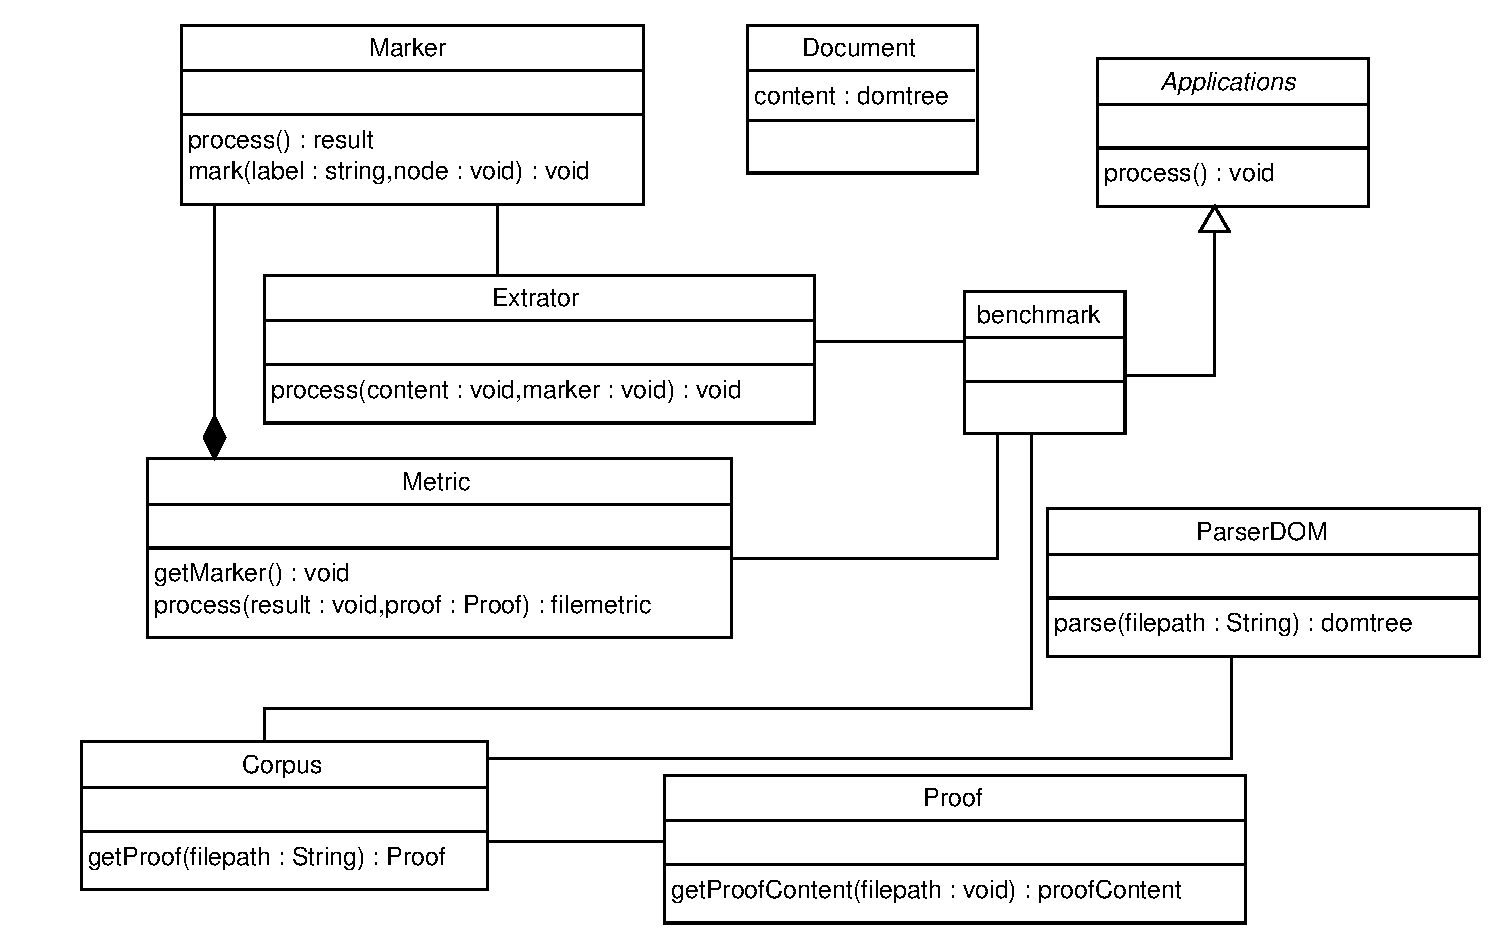
\includegraphics[width=12cm]{img/classes.eps}
  \caption{x}
  \label{x}
  \end{center}
\end{figure}

Observando os passos necessários para que seja possível o inicio do
desenvolvimento de uma solução de experimentação fica evidente a
necessidade de um módulo capaz de corrigir problemas de
codificação nos documentos e má formação seguindo da uma estrutura em
memória para que seja possível trabalhar neste documento. Por esse
motivo, o primeiro módulo descrito é o Parser que atende a essa
necessidade, sendo descrio a seguir:

\begin{verbatim}
- Parser: 
  - ForceEncode:
    Normaliza a codificação de um documento para
    UTF-8.
  - Santizer:
    Verifica a corretude do documento HTML e
    corrige alguns erros e problemas comulmente
    encontrados.
  - ParserDOM:
    Transforma o documento em uma estrutura em
    memória DOM, essa estutura é recomendada
    para a representação de documentos HTML
    em memória pela W3C.
\end{verbatim}

Com o documento HTML em memória e disponível para a execução de rotinas
sobre sua estrutura a forma como as rotinas irão guardar seus resultados
é importante, pois determinará todo o processo de geração de resultados
e avaliação. Com isso, descrevemos o módulo de ''anotação'' e a interface
que todas as rotinas, denominadas extratores, devem atender.

Existe uma peculariedade com a modelagem adotada, pois a forma de marcar
o resultado influencia como esse resultado poderá ser avaliado, porém
essa dependecia será descrita quando for descrito o módulo de avaliação.

\begin{verbatim}
- Marcadores:
  Armazena nós em rótulos para que eles possam ser
  organizados ou segmentados.

- Extratores:
  Procura por elementos que atendem a especificação
  de um rótulo em um documento e o marca, utilizando
  o marcador, com o referido rótulo.
\end{verbatim}

O conjunto de módulos descritos até então fornece um conjunto de
funcionalidades que proporciona a colocação da solução encontrada em
prática, porém como o objetivo da ferramenta é proporcionar um ambiente
de experimentação são necessários mais alguns módulos, esses com o
objetivo direto a tarefa de experimentação.

A capacidade de avaliar os algoritmos, ou soluções, propostos é muito
importante. Por isso, o módulo de avaliação fornece o conjunto de regras
para que o resultado obtido possa ser mensurado e retornado como
informações estatistica. A formas de avaliar são diretamente
relacionadas a forma que o resultado foi armazenada, então para cada
avaliador existe um marcador disponível, pois esse marcador armazena a
solução no formato adequado para ser avalido posteriormente.

Além de um marcador o avaliador necessita também de uma fonte de
informação correta, denominada gabarito. Esse gabarito fornece um
conjunto de informação, no mesmo formato que o conjunto armazenado pelo
marcador, para que seja possível o cruzamento de informação para a
avaliação. Um formato básico que atende as principais tarefas de
identificação em páginas HTML é fornecido como base junto a ferramenta.

\begin{verbatim}
- Avaliador:
  Recebe os rótulos, junto aos conjunto de nós
  que pertencem a eles, e também o gabarito para
  quantificar a qualidade do extrator.

- Gabarito: 
  Armazena os rótulos, junto ao conjunto de nós
  de cada rótulo, para que os extratores possam
  ser avaliados.
\end{verbatim}

A experimentação normalmente ocorre sobre um grande conjunto de
documentos, por esse motivo descrevemos uma estrutura que descreve esse
conjunto, denominado corpus. O corpus descreve um conjunto de
documentos, informando a natureza dos documentos, o tipo de gabarito que
pode ser obtido dos documentos e para quais tarefas esses documentos são
interessantes.

\begin{verbatim}
- Corpus: 
  Conjunto de documentos, junto aos seus gabaritos.
  Os corpus são descritos por um arquivo de
  configuração que especifica o tipo de gabarito
  que esse corpus pode produzir e quais as tarefas
  que ele pode ser utilizado.
\end{verbatim}

Para utilizar desses módulos podem ser implementadas aplicações que
utilizam o que é mais interessante para ela. Um bom exemplo de aplicação
é a geração de um relatório de desempenho (Benchmark) para o conjunto de
extratores e corpus. Atualmente o benchmark é a unica aplicação
disponível junto a ferramenta, pois essa é uma necessidade direta para a
experimentação. A seguir é apresentado um diagrama de sequência para
exemplificar a utilização da ferramenta.

\begin{figure}[htb!]
  \begin{center}
  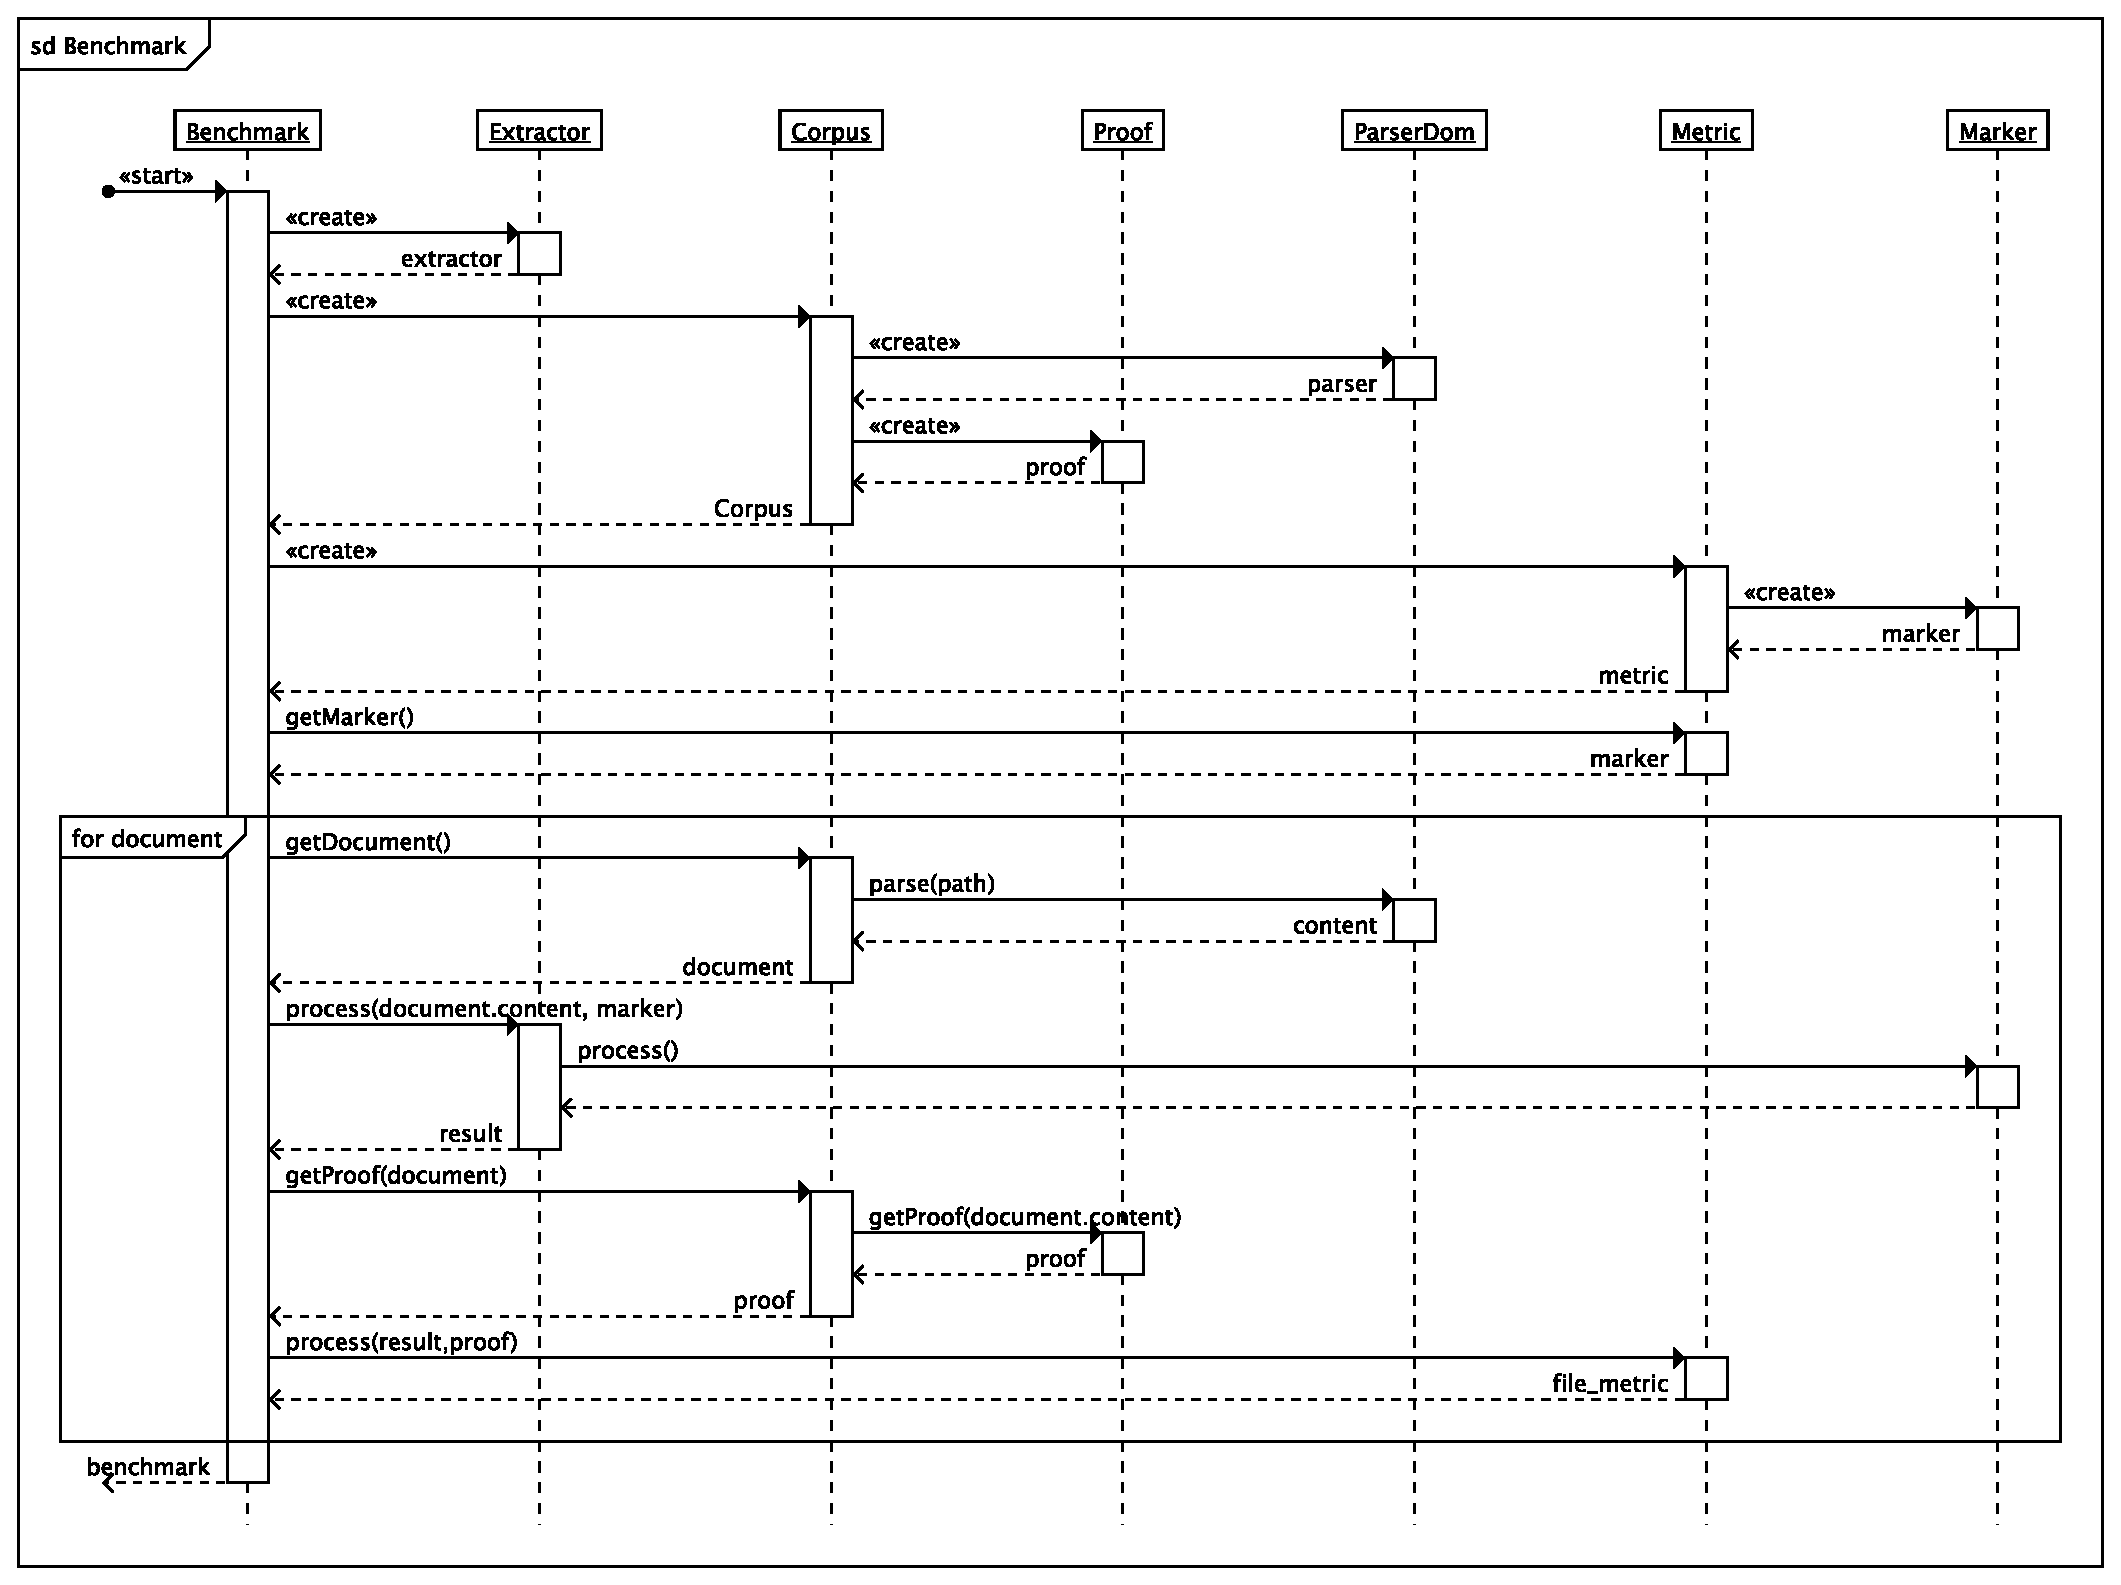
\includegraphics[width=14cm]{img/fastbenchmark.eps}
  \caption{x}
  \label{x}
  \end{center}
\end{figure}

  \subsection{Acompanhamento do Desenvolvimento da Ferramenta}
%- mini-acompanhamento da execução: seqüência de tarefas de desenvolvimento utilizadas junto com estatísticas de tempo e esforço por tarefa.
\begin{enumerate}
\item Definição da Tarefa: 1 de agosto a 30 de agosto. \\
Inicialmente foi realizada uma busca pelos trabalhos relacionados a
extração de elementos e marcação em páginas Web para engrandecer o
conhecimento sobre a área, melhorando a capacidade de entendimento
sobre o problema.

\item Modelagem do Problema: 1 de setembro a 15 de setembro. \\ 
Após conhecer bem o problema de segmentação e marcação de elementos em
páginas Web a modelagem de uma ferramenta de apoio se tornou possível.
Durante esse processo de modelagem foram estabelecidos os limites e as
necessidades de uma ferramenta para suporte a criação de soluções para
o problema.

\item Impementação do Framework e Testes: 15 de setembro a 30 de
novembro. \\
Durante o mês de setembro, outubro e novembro foi realizada a
codificação da ferramenta modelada. Durante esse tempo também foram
desenvolvidos alguns testes unitários para garantir a qualidade do
desenvolvimento da aplicação. Além do desenvolvimento da ferramenta de
suporte, também foi realizada a tentativa de resolver uma tarefa de
segmentação. Essa tarefa é detalhado mais adiante no texto, assim como
seus resultados.

\item Documentação de usuario e relatório: 30 de novembro a 15 de
dezembro. \\
Os últimos 15 dias de projeto foram utilizados para a elaboração deste
documento e também para a criação da documentação para usuários,
tornando a ferramenta fácil de ser utilizada por profissíonais que
queiram pesquisar sobre problemas que possam ser modelados de forma
similar, ou seja, problemas de segmentação ou detecção de elementos em
páginas HTML.
\end{enumerate}

%\section{Especificação}
%- especificação do programa
% - objetivos, requisitos
% - diagramas de especificação, por exemplo use-cases.
\remove{
	- Para facilitar agilizar e promover uma fácil abordagem sobre tarefas
  de experimentação em páginas HTML é necessário um framework que
  possibilite: \\
		- parsear uma página HTML para uma árvore DOM: preprocessamento... \\
		- Criar um pipe onde módulos possam ser aplicados sobre a árvore DOM
    \\
		- fornecer uma interface onde os resultados dos módulos são
    guardados \\
		- Criar uma interface onde regras de avaliação sobre o resultado
    possam ser aplicadas \\
		- Criar forma de criar gabaritos para que as métricas de avaliação
    possam ser automatizadas \\
}

%\section{Modelagem}
%- projeto modular do programa
% - critérios de projeto utilizados
% - diagramas de arquitetura e/ou segmentação do programa, por     exemplo UML.
% - organização do programa (componentes, módulos, classes,...),    por exemplo  diagramas de classe UML.
% - diagramas de organização dos dados, por exemplo diagramas     de modelagem de dados, ou entidade e relacionamentos.

\remove{
- Modulos \\
 A organização modular do projeto facilita o entendimento da ferramenta
 e possibilita que correções e atualizações possam ser feitas
 facilmente. Abaixo descrevemos os principais módulos da ferramenta:

 Extratores: \\
  Conjunto de classes que são especializadas em extrair informação de
  árvores DOM e utilizando {\bf Marcadores} rotular cada tipo de
  informação extraida.

 Marcadore: \\
  Conjunto de classes especialzadas em atribuir labels a nós da árvore
  DOM. Faz-se necessário deixar o desenvolvimento desse módulo
  independente, pois a variação na forma de avaliação pelas {\bf
  Métricas} influência a forma que os nós devem ser marcados.

 Métricas (Avaliadores): \\
  Os avaliadores atribuem valores para o acerto e o erro nas marcações.
  Cada tarefa pode ser avaliada de forma diretente, pois é diretamente
  relacionado a abordagem da tarefa ao tipo de avaliação. No final a
  Métrica retorna três valores que são comulmente utilizados no universo
  de aprendizado de máquina e experimentação (recall, precision,
  f-measure), sendo documentada a forma do cálculo desses valores dentro
  do módulo.
 
 Aplicativos: \\
  Os aplicativos são agrupados para agilizar e facilitar a utilização da
  ferramenta pelos usuários. Nesse módulo são encontradas as aplicações
  da ferrameta proposta, como: benchmarks e geradores de recortes com os
  diversos extratores.
}
\subsection{Código Fonte}

Para a codificação da ferramenta foi escolhida a linguagem script
Python. Sua facilidade de prototipação e programação foram pontos
positivos para essa escolha.

Para tornar o código claro e padronizado foram utilizadas as
recomendações de codificação da empresa Fast.
Isso porque, as normas apresentadas são próximas as utilizadas pelos 
próprios módulos disponibilizados nas bibliotecas padrões e, além disso,
esclarecem pontos que muitas vezes ficam dúbios em outros manuais de 
recomendações para codificação em Python. Porém,
  o documento contendo as recomendações e regras não
  poderá ser anexado por causa dos termos de sigilo. 

Todo o código esta comentado no formato recomendado pelo manual de
referência de Python e o  módulo de geração de documentação automático
PyDoc foi utilizado, gerando a documentação em formato HTML. Para a
documentação do código também foi adotado, como adendo, o padrão de 
descrição de comentário recomentado pela empresa Fast.

\subsection{Validação e Testes}
%- testes dos modulos implementados

Para verificar o funcionamento da ferramenta e validar a modelagem apresentada a tarefa de identificação de tabelas genuinas foi escolhida. Utilizando a Ferramenta de Experimentação em Documentos HTML foi implementada uma abordagem simplificada a proposta em []. Mesmo não obtendo bons resultados para a tarefa o objetivo foi alcançado, já que a ferramenta proporcionou a rápida codificação e experimentação da tarefa. Esses resultados estão disponíveis no apendice X e um fragmento do corpus utilizado está disponível junto ao código para a realizações de testes pelo usuário.

Foi utilizado o framework de teste unitários fornecido pela distribuição
oficial do Python [1]. Os módulos foram testados, buscando a verificação
da corretude do código e também foram criados testes para verificar a
API das classes importantes para a ferramenta.

Os testes e todos os logs podem ser verificados no Anexo X. Esses testes
também se encontram junto ao código, sendo eles nomeados como
test\_<nome\_do\_arquivo>.py e podem ser executados separadamento como
um scripts Python.

A cobertura do código por testes foi programada a partir do modelo de
sequência da aplicação "Benchmark" que descreve o principal uso da
ferramenta. Outros casos também foram verificados para garantir que
módulos de suporte, como o parser DOM ou a algorítmos clássicos como
distáncia de ediçao, DFS, LLC estão corretamete
implementados.

\subsection{Documentação do Usuário}

A documentação para utilização das aplicações existentes na ferramenta
se encontram junto ao código e são apresentadas quando o usuário
solicita ajuda (help) pela linha de comando. Essa documentação foi
criada utilizando a biblioteca optparser, também disponibilizada pela
distribuição oficial de Python.

\remove{
A documentação do código foi realizada utilizando outro modelo padrão de
Python, o pydoc, e pode ser encontrada na pasta raiz do projeto em
formato HTML para facilitar a leitura e a busca por alguma
funcionalidade específica.
}

\subsection{Conteúdo do CD}

O CD-ROM engtregue, onde esse documento pode ser encontrado, contêm
todos os arquivos fonte e documentos necessários para o entendimento e
utilização da ferramenta. Também é fornecido um pequeno conjunto de
documentos onde a tarefa de detecção de tabela genuida pode ser
executada e os resultados analizados utilizando a aplicação de Benchmark.

A Estrutura de diretórios do código fonte, que pode ser encontrada na
pasta sorce, é a seguinte:

\begin{verbatim}
|-- source
  |-- README.txt 
  |-- __init__.py
  |-- apps
  |   |-- __init__.py
  |   |-- benchmark.py
  |   |-- config_example.cnf
  |   |-- configurator.py
  |   |-- fastbenchmark.py
  |   |-- out
  |   |-- test_.py
  |   |-- test_benchmark.py
  |   `-- test_configurator.py
  |-- corpus.py
  |-- extractors
  |   |-- __init__.py
  |   `-- distancebypair
  |       |-- __init__.py
  |       |-- coloring.py
  |       |-- distancebypairbase.py
  |       |-- node.py
  |       |-- table.py
  |       `-- test_node.py
  |-- markerbase.py
  |-- markercoloring.py
  |-- metricbase.py
  |-- metrictables.py
  |-- tablesproof.py
  |-- test_corpus.py
  `-- utils
      |-- __init__.py
      |-- distances.py
      |-- dynamicimport.py
      |-- forceencode.py
      |-- parsedom.py
      |-- sanitizer.py
      |-- test_distances.py
      |-- test_dynamicimport.py
      |-- test_forceencode.py
      `-- test_parsedom.py
\end{verbatim}

Na pasta pydoc pode ser encontrado a documentação gerada automaticamente
a partir do código.

\begin{verbatim}
|-- pydoc
|   |-- __init__.html
|   |-- configurator.html
|   |-- distancebypairbase.html
|   |-- distances.html
|   |-- dynamicimport.html
|   |-- fastbenchmark.html
|   |-- forceencode.html
|   |-- markerbase.html
|   |-- markercoloring.html
|   |-- metricbase.html
|   |-- node.html
|   |-- sanitizer.html
|   |-- table.html
|   |-- tablesproof.html
|   |-- test_configurator.html
|   |-- test_distances.html
|   |-- test_dynamicimport.html
|   `-- test_parsedom.html
\end{verbatim}

Na pasta corpus, o sample para a execução e teste do benchmark pode ser
encontrado:

\begin{verbatim}
|-- corpus
    |-- file0.html 
    |
    `-- filen.html
\end{verbatim}

Para exemplificar o resultado de um Benchmark em um conjunto real de
documentos e o tempo de execução, um corpus utilizado em estudos da área,
foi adicionado ao CD-ROM a pasta experimento.

\begin{verbatim}
|-- experiments
  |-- benchmark100docs.csv
  |-- outAndtime100docs.out
  |-- benchmark300docs.csv
  |-- outAndtime300docs.out
  |-- benchmark600documentos.csv
  `-- outAndtime600docs.out
\end{verbatim}
%      - documentação para o usuário 

% \balancecolumns

\bibliographystyle{alpha}
\bibliography{bib}
\end{document}
